% Options for packages loaded elsewhere
\PassOptionsToPackage{unicode}{hyperref}
\PassOptionsToPackage{hyphens}{url}
%
\documentclass[
]{book}
\usepackage{lmodern}
\usepackage{amsmath}
\usepackage{ifxetex,ifluatex}
\ifnum 0\ifxetex 1\fi\ifluatex 1\fi=0 % if pdftex
  \usepackage[T1]{fontenc}
  \usepackage[utf8]{inputenc}
  \usepackage{textcomp} % provide euro and other symbols
  \usepackage{amssymb}
\else % if luatex or xetex
  \usepackage{unicode-math}
  \defaultfontfeatures{Scale=MatchLowercase}
  \defaultfontfeatures[\rmfamily]{Ligatures=TeX,Scale=1}
\fi
% Use upquote if available, for straight quotes in verbatim environments
\IfFileExists{upquote.sty}{\usepackage{upquote}}{}
\IfFileExists{microtype.sty}{% use microtype if available
  \usepackage[]{microtype}
  \UseMicrotypeSet[protrusion]{basicmath} % disable protrusion for tt fonts
}{}
\makeatletter
\@ifundefined{KOMAClassName}{% if non-KOMA class
  \IfFileExists{parskip.sty}{%
    \usepackage{parskip}
  }{% else
    \setlength{\parindent}{0pt}
    \setlength{\parskip}{6pt plus 2pt minus 1pt}}
}{% if KOMA class
  \KOMAoptions{parskip=half}}
\makeatother
\usepackage{xcolor}
\IfFileExists{xurl.sty}{\usepackage{xurl}}{} % add URL line breaks if available
\IfFileExists{bookmark.sty}{\usepackage{bookmark}}{\usepackage{hyperref}}
\hypersetup{
  pdftitle={STAT 234: Data Science},
  pdfauthor={Matt Higham},
  hidelinks,
  pdfcreator={LaTeX via pandoc}}
\urlstyle{same} % disable monospaced font for URLs
\usepackage{color}
\usepackage{fancyvrb}
\newcommand{\VerbBar}{|}
\newcommand{\VERB}{\Verb[commandchars=\\\{\}]}
\DefineVerbatimEnvironment{Highlighting}{Verbatim}{commandchars=\\\{\}}
% Add ',fontsize=\small' for more characters per line
\usepackage{framed}
\definecolor{shadecolor}{RGB}{248,248,248}
\newenvironment{Shaded}{\begin{snugshade}}{\end{snugshade}}
\newcommand{\AlertTok}[1]{\textcolor[rgb]{0.94,0.16,0.16}{#1}}
\newcommand{\AnnotationTok}[1]{\textcolor[rgb]{0.56,0.35,0.01}{\textbf{\textit{#1}}}}
\newcommand{\AttributeTok}[1]{\textcolor[rgb]{0.77,0.63,0.00}{#1}}
\newcommand{\BaseNTok}[1]{\textcolor[rgb]{0.00,0.00,0.81}{#1}}
\newcommand{\BuiltInTok}[1]{#1}
\newcommand{\CharTok}[1]{\textcolor[rgb]{0.31,0.60,0.02}{#1}}
\newcommand{\CommentTok}[1]{\textcolor[rgb]{0.56,0.35,0.01}{\textit{#1}}}
\newcommand{\CommentVarTok}[1]{\textcolor[rgb]{0.56,0.35,0.01}{\textbf{\textit{#1}}}}
\newcommand{\ConstantTok}[1]{\textcolor[rgb]{0.00,0.00,0.00}{#1}}
\newcommand{\ControlFlowTok}[1]{\textcolor[rgb]{0.13,0.29,0.53}{\textbf{#1}}}
\newcommand{\DataTypeTok}[1]{\textcolor[rgb]{0.13,0.29,0.53}{#1}}
\newcommand{\DecValTok}[1]{\textcolor[rgb]{0.00,0.00,0.81}{#1}}
\newcommand{\DocumentationTok}[1]{\textcolor[rgb]{0.56,0.35,0.01}{\textbf{\textit{#1}}}}
\newcommand{\ErrorTok}[1]{\textcolor[rgb]{0.64,0.00,0.00}{\textbf{#1}}}
\newcommand{\ExtensionTok}[1]{#1}
\newcommand{\FloatTok}[1]{\textcolor[rgb]{0.00,0.00,0.81}{#1}}
\newcommand{\FunctionTok}[1]{\textcolor[rgb]{0.00,0.00,0.00}{#1}}
\newcommand{\ImportTok}[1]{#1}
\newcommand{\InformationTok}[1]{\textcolor[rgb]{0.56,0.35,0.01}{\textbf{\textit{#1}}}}
\newcommand{\KeywordTok}[1]{\textcolor[rgb]{0.13,0.29,0.53}{\textbf{#1}}}
\newcommand{\NormalTok}[1]{#1}
\newcommand{\OperatorTok}[1]{\textcolor[rgb]{0.81,0.36,0.00}{\textbf{#1}}}
\newcommand{\OtherTok}[1]{\textcolor[rgb]{0.56,0.35,0.01}{#1}}
\newcommand{\PreprocessorTok}[1]{\textcolor[rgb]{0.56,0.35,0.01}{\textit{#1}}}
\newcommand{\RegionMarkerTok}[1]{#1}
\newcommand{\SpecialCharTok}[1]{\textcolor[rgb]{0.00,0.00,0.00}{#1}}
\newcommand{\SpecialStringTok}[1]{\textcolor[rgb]{0.31,0.60,0.02}{#1}}
\newcommand{\StringTok}[1]{\textcolor[rgb]{0.31,0.60,0.02}{#1}}
\newcommand{\VariableTok}[1]{\textcolor[rgb]{0.00,0.00,0.00}{#1}}
\newcommand{\VerbatimStringTok}[1]{\textcolor[rgb]{0.31,0.60,0.02}{#1}}
\newcommand{\WarningTok}[1]{\textcolor[rgb]{0.56,0.35,0.01}{\textbf{\textit{#1}}}}
\usepackage{longtable,booktabs}
\usepackage{calc} % for calculating minipage widths
% Correct order of tables after \paragraph or \subparagraph
\usepackage{etoolbox}
\makeatletter
\patchcmd\longtable{\par}{\if@noskipsec\mbox{}\fi\par}{}{}
\makeatother
% Allow footnotes in longtable head/foot
\IfFileExists{footnotehyper.sty}{\usepackage{footnotehyper}}{\usepackage{footnote}}
\makesavenoteenv{longtable}
\usepackage{graphicx}
\makeatletter
\def\maxwidth{\ifdim\Gin@nat@width>\linewidth\linewidth\else\Gin@nat@width\fi}
\def\maxheight{\ifdim\Gin@nat@height>\textheight\textheight\else\Gin@nat@height\fi}
\makeatother
% Scale images if necessary, so that they will not overflow the page
% margins by default, and it is still possible to overwrite the defaults
% using explicit options in \includegraphics[width, height, ...]{}
\setkeys{Gin}{width=\maxwidth,height=\maxheight,keepaspectratio}
% Set default figure placement to htbp
\makeatletter
\def\fps@figure{htbp}
\makeatother
\setlength{\emergencystretch}{3em} % prevent overfull lines
\providecommand{\tightlist}{%
  \setlength{\itemsep}{0pt}\setlength{\parskip}{0pt}}
\setcounter{secnumdepth}{5}
\usepackage{booktabs}
\usepackage{amsthm}
\makeatletter
\def\thm@space@setup{%
  \thm@preskip=8pt plus 2pt minus 4pt
  \thm@postskip=\thm@preskip
}
\makeatother
\ifluatex
  \usepackage{selnolig}  % disable illegal ligatures
\fi
\usepackage[]{natbib}
\bibliographystyle{apalike}

\title{STAT 234: Data Science}
\author{Matt Higham}
\date{2021-05-12}

\begin{document}
\maketitle

{
\setcounter{tocdepth}{1}
\tableofcontents
}
\hypertarget{course-description}{%
\chapter{Course Description}\label{course-description}}

Describe course, maybe give information on \texttt{R\ Studio} server.

This is a \emph{sample} book written in \textbf{Markdown}. You can use anything that Pandoc's Markdown supports, e.g., a math equation \(a^2 + b^2 = c^2\).

The \textbf{bookdown} package can be installed from CRAN or Github:

Remember each Rmd file contains one and only one chapter, and a chapter is defined by the first-level heading \texttt{\#}.

\hypertarget{intro}{%
\chapter{\texorpdfstring{Introduction: Getting Started with \texttt{R} and \texttt{R\ Studio}}{Introduction: Getting Started with R and R Studio}}\label{intro}}

Figures and tables with captions will be placed in \texttt{figure} and \texttt{table} environments, respectively.

\begin{Shaded}
\begin{Highlighting}[]
\FunctionTok{par}\NormalTok{(}\AttributeTok{mar =} \FunctionTok{c}\NormalTok{(}\DecValTok{4}\NormalTok{, }\DecValTok{4}\NormalTok{, .}\DecValTok{1}\NormalTok{, .}\DecValTok{1}\NormalTok{))}
\FunctionTok{plot}\NormalTok{(pressure, }\AttributeTok{type =} \StringTok{\textquotesingle{}b\textquotesingle{}}\NormalTok{, }\AttributeTok{pch =} \DecValTok{19}\NormalTok{)}
\end{Highlighting}
\end{Shaded}

\begin{figure}

{\centering 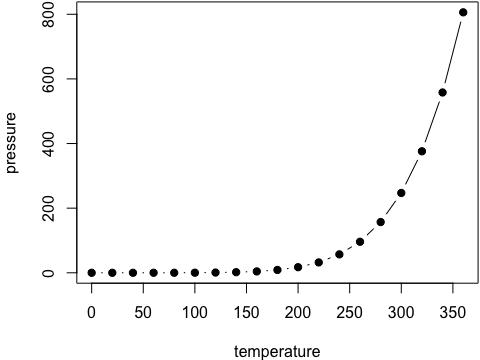
\includegraphics[width=0.8\linewidth]{01-intro_files/figure-latex/nice-fig-1} 

}

\caption{Here is a nice figure!}\label{fig:nice-fig}
\end{figure}

\textbf{Goals}:

\begin{enumerate}
\def\labelenumi{\arabic{enumi}.}
\item
  Use \texttt{R\ Studio} on the server
\item
  Use \texttt{R\ Markdown} and code chunks
\item
  Load in data to \texttt{R\ Studio}
\item
  Run code and change a few things within that code
\item
  Correct some common errors when running code in \texttt{R}
\end{enumerate}

\textbf{Note}: If you are using a downloaded version of \texttt{R\ Studio} because you already have it on your computer from Spring 2020, then you'll need to install the \texttt{rmdformats} package. If you're using the server, then ignore this note :)

\hypertarget{intro-to-r-and-r-studio}{%
\section{\texorpdfstring{Intro to \texttt{R} and \texttt{R\ Studio}}{Intro to R and R Studio}}\label{intro-to-r-and-r-studio}}

\texttt{R} is a statistical computing software used by many statisticians as well as professionals in other fields, such as biology, ecology, business, and psychology. The goal of Week 0 is to provide basic familiarity with \texttt{R} and \texttt{R\ Markdown}, which we will be using for the entire semester.

\begin{center}\rule{0.5\linewidth}{0.5pt}\end{center}

Open \texttt{R\ Studio} on the SLU \texttt{R\ Studio} server at \url{http://rstudio.stlawu.local:8787} and create a folder called STAT\_234 or some other meaningful title to you. Note that you must be on campus to use the \texttt{R\ Studio} server, unless you use a VPN. Directions on how to set-up VPN are \url{https://infotech.stlawu.edu/support/content/11269} for Macs and \url{https://stlawu.teamdynamix.com/TDClient/1805/Portal/KB/ArticleDet?ID=55118} for Windows.

Next, create a subfolder within your STAT\_234 folder. Title it \emph{Notes} (or whatever you want really).

Then, create an \texttt{R\ Project} by Clicking File -\textgreater{} New Project -\textgreater{} New Directory. Name the new project Week0\_R\_Intro (or some other meaningful title to you) and put it in the Notes folder. We will make a new project for each topic of class, for each homework assignment that requires the use of \texttt{R}, and for each project we have in class.

After the project is created, download the \emph{Week0\_IntroR.zip} file found on Sakai (in Resources) to your folder with the new project. Then, you can upload that file in to the server by clicking ``Upload'' in the bottom right panel. In the dialog box that appears, you can click ``Choose File'' and navigate to the folder where you saved the .Rmd file (probably Downloads by default). The zip file will automatically expand once uploaded. It includes a .Rmd file, a .html file, and two .csv data sets.

Once you upload the file, click on it to open it and scroll down to this line.

\textbf{From this point forward, I recommend following along with the .Rmd file that you just opened}. Reading this type of file takes a little bit of getting used to, but I think it's easier than trying to jump back and forth between the .Rmd and .html file.

Before moving on, click the \textbf{Knit} button in the top-left window at the top of the menu bar (look for the knitting needle icon). Make sure that the file knits to a pretty-looking .html file. This .html file is the same as the one that you've been reading along with so far. The newly knitted .html file can now be found in your folder with your \texttt{R} project.

\begin{center}\rule{0.5\linewidth}{0.5pt}\end{center}

\hypertarget{what-are-r-r-studio-and-r-markdown}{%
\section{\texorpdfstring{What are \texttt{R}, \texttt{R\ Studio}, and \texttt{R\ Markdown}?}{What are R, R Studio, and R Markdown?}}\label{what-are-r-r-studio-and-r-markdown}}

The distinction between the 3 will become more clear later on. For now,

\begin{itemize}
\item
  \texttt{R} is a statistical coding software used heavily for data analysis and statistical procedures.
\item
  \texttt{R\ Studio} is a nice IDE (Integrated Development Environment) for \texttt{R} that has a lot of convenient features. Think of this as just a convenient User Interface.
\item
  \texttt{R\ Mardkown} allows users to mix regular Microsoft-Word-style text with code. The \texttt{.Rmd} file ending denotes an \texttt{R\ Mardkown} file. \texttt{R\ Markdown} has many options that we will use heavily throughout the semester, but there's no need to worry about these now.
\end{itemize}

\begin{center}\rule{0.5\linewidth}{0.5pt}\end{center}

\hypertarget{r-packages-and-the-tidyverse}{%
\paragraph{\texorpdfstring{\texttt{R} Packages and the \texttt{tidyverse}}{R Packages and the tidyverse}}\label{r-packages-and-the-tidyverse}}

You can think of \texttt{R} packages as add-ons to \texttt{R} that let you do things that \texttt{R} on its own would not be able to do. If you're in to video games, you can think of \texttt{R} packages as extra Downloadable Content (DLC). But, unlike most gaming DLC, \texttt{R} packages are always free and we will make very heavy use of \texttt{R} packages.

The \texttt{tidyverse} is a series of \texttt{R} packages that are useful for data science. In the order that we will encounter them in this class, the core \texttt{tidyverse} packages are:

\begin{enumerate}
\def\labelenumi{\arabic{enumi}.}
\tightlist
\item
  \texttt{ggplot2} for plotting data
\item
  \texttt{dplyr} for data wrangling and summarizing
\item
  \texttt{tidyr} for data tidying and reshaping
\item
  \texttt{readr} for data import
\item
  \texttt{tibble} for how data is stored
\item
  \texttt{stringr} for text data
\item
  \texttt{forcats} for factor (categorical) data
\item
  \texttt{purrr}, for functional programming, the only one of these core 8 that we won't get to use
\end{enumerate}

We will use packages outside of the core \texttt{tidyverse} as well, but the \texttt{tidyverse} is the main focus.

\begin{center}\rule{0.5\linewidth}{0.5pt}\end{center}

\hypertarget{putting-code-in-a-.rmd-file}{%
\paragraph{\texorpdfstring{Putting Code in a \texttt{.Rmd} File}{Putting Code in a .Rmd File}}\label{putting-code-in-a-.rmd-file}}

We are going to change one option before proceeding. In the top file menu, click Tools -\textgreater{} Global Options -\textgreater{} R Markdown and then uncheck the box that says ``Show output inline for all R Markdown documents''. Don't worry about this for now, but changing this option just means that code results will appear in the bottom-left window and graphs will appear in the bottom-right window of \texttt{R\ Studio}.

Up to this point, we have only had text in our .Rmd file. The first thing that we will do that involves code is to load a package into \texttt{R} with the \texttt{library()} function. A package is just an \texttt{R} add-on that lets you do more than you could with just \texttt{R} on its own. Load the \texttt{tidyverse} package into \texttt{R} by typing and running the \texttt{library(tidyverse)} line. You can run code by placing your cursor in the line of code and

\begin{enumerate}
\def\labelenumi{\arabic{enumi}.}
\item
  Clicking the ``Run'' button in the menu bar of the top-left window of \texttt{R\ Studio} or
\item
  (Recommended) Clicking ``Command + Enter'' on a Mac or ``Control + Enter'' on a PC.
\end{enumerate}

Note that all code (like what appears in the following lines) appears in grey boxes surrounded by three backticks while normal text (like what you are reading now) has a white background with no backticks.

\begin{Shaded}
\begin{Highlighting}[]
\FunctionTok{library}\NormalTok{(tidyverse)}
\end{Highlighting}
\end{Shaded}

\begin{verbatim}
## -- Attaching packages --------------------------------------- tidyverse 1.3.0 --
\end{verbatim}

\begin{verbatim}
## v ggplot2 3.3.3     v purrr   0.3.4
## v tibble  3.1.1     v dplyr   1.0.4
## v tidyr   1.1.2     v stringr 1.4.0
## v readr   1.3.1     v forcats 0.5.0
\end{verbatim}

\begin{verbatim}
## -- Conflicts ------------------------------------------ tidyverse_conflicts() --
## x dplyr::filter() masks stats::filter()
## x dplyr::lag()    masks stats::lag()
\end{verbatim}

When you run the following line, some text will appear in the bottom-left window. We won't worry too much about what this text means now, but we also won't ignore it completely. You should be able to spot the 8 core \texttt{tidyverse} packages listed above as well as some numbers that follow each package. The numbers correspond to the package version. There's some other things too, but as long as this text does not start with ``Error:'', you're good to go!

Congrats on running your first line of code for this class! This particular code isn't particularly exciting because it doesn't really do anything that we can see.

We have run \texttt{R} code using an \texttt{R} chunk. While most of this document is text (not \texttt{R} code), the text inside the three opening quotation marks is \texttt{R} code. Try making your own \texttt{R} chunk below by clicking \textbf{Insert} (the green button in the top left window) -\textgreater{} R. In your \texttt{R} chunk, perform the calculation \texttt{99\ +\ 10} by typing \texttt{99\ +\ 10} into your code chunk and pressing Command + Enter or Control + Enter.

So, that still wasn't super exciting. \texttt{R} can perform basic calculations, but you could just use a calculator or Excel for that. In order to look at things that are a bit more interesting, we need some data.

\begin{center}\rule{0.5\linewidth}{0.5pt}\end{center}

\hypertarget{alcohol-data}{%
\section{Alcohol Data}\label{alcohol-data}}

We will be looking at two data sets just to get a little bit of a preview of things we will be working on for the rest of the semester. \textbf{Important}: Do not worry about understanding what all of this code is doing at this point. There will be plenty of time to understand this in the weeks ahead. The purpose of this section is just to get used to using \texttt{R}: there will be more detailed videos, explanations, and exercises about the functions used and various options in the coming weeks. In particular, the following code uses the \texttt{ggplot2}, \texttt{dplyr}, and \texttt{tidyr} packages, which we will cover in detail throughout the first \textasciitilde{} 4 weeks of this course.

Data for this first part was obtained from fivethirtyeight at the following link: \url{https://github.com/fivethirtyeight/data/tree/master/alcohol-consumption}

The first step is to read the data set into \texttt{R}. Though you have already downloaded alcohol.csv, we still need to load it into \texttt{R}. Check to make sure the alcohol.csv is in the Files pane of your bottom-right hand window. Then, run the following line by placing your cursor in the line below and clicking Cmd + Enter or Control + Enter:

\begin{Shaded}
\begin{Highlighting}[]
\FunctionTok{read\_csv}\NormalTok{(}\StringTok{"alcohol.csv"}\NormalTok{)}
\end{Highlighting}
\end{Shaded}

Note that we do not need the full file extension \textbf{if} we have the data set in an \texttt{R} project.

Did something show up in your console window? If so, great! If not, make sure that the data set is in your \texttt{R} project folder.

We would like to name our data set something so that we could easily reference it later, so name your data set using the \texttt{\textless{}-} operator, as in

\begin{Shaded}
\begin{Highlighting}[]
\NormalTok{alcohol\_data }\OtherTok{\textless{}{-}} \FunctionTok{read\_csv}\NormalTok{(}\StringTok{"alcohol.csv"}\NormalTok{)}
\FunctionTok{head}\NormalTok{(alcohol\_data)}
\end{Highlighting}
\end{Shaded}

\begin{verbatim}
## # A tibble: 6 x 5
##   country      beer_servings spirit_servings wine_servings total_litres_of_pure~
##   <chr>                <dbl>           <dbl>         <dbl>                 <dbl>
## 1 Afghanistan              0               0             0                   0  
## 2 Albania                 89             132            54                   4.9
## 3 Algeria                 25               0            14                   0.7
## 4 Andorra                245             138           312                  12.4
## 5 Angola                 217              57            45                   5.9
## 6 Antigua & B~           102             128            45                   4.9
\end{verbatim}

Reference a figure by its code chunk label with the \texttt{fig:} prefix, e.g., see Figure \ref{fig:nice-fig}. Similarly, you can reference tables generated from \texttt{knitr::kable()}, e.g., see Table \ref{tab:nice-tab}.

\begin{Shaded}
\begin{Highlighting}[]
\NormalTok{knitr}\SpecialCharTok{::}\FunctionTok{kable}\NormalTok{(}
  \FunctionTok{head}\NormalTok{(iris, }\DecValTok{20}\NormalTok{), }\AttributeTok{caption =} \StringTok{\textquotesingle{}Here is a nice table!\textquotesingle{}}\NormalTok{,}
  \AttributeTok{booktabs =} \ConstantTok{TRUE}
\NormalTok{)}
\end{Highlighting}
\end{Shaded}

\begin{table}

\caption{\label{tab:nice-tab}Here is a nice table!}
\centering
\begin{tabular}[t]{rrrrl}
\toprule{}
Sepal.Length & Sepal.Width & Petal.Length & Petal.Width & Species\\
\midrule{}
5.1 & 3.5 & 1.4 & 0.2 & setosa\\
4.9 & 3.0 & 1.4 & 0.2 & setosa\\
4.7 & 3.2 & 1.3 & 0.2 & setosa\\
4.6 & 3.1 & 1.5 & 0.2 & setosa\\
5.0 & 3.6 & 1.4 & 0.2 & setosa\\
\addlinespace
5.4 & 3.9 & 1.7 & 0.4 & setosa\\
4.6 & 3.4 & 1.4 & 0.3 & setosa\\
5.0 & 3.4 & 1.5 & 0.2 & setosa\\
4.4 & 2.9 & 1.4 & 0.2 & setosa\\
4.9 & 3.1 & 1.5 & 0.1 & setosa\\
\addlinespace
5.4 & 3.7 & 1.5 & 0.2 & setosa\\
4.8 & 3.4 & 1.6 & 0.2 & setosa\\
4.8 & 3.0 & 1.4 & 0.1 & setosa\\
4.3 & 3.0 & 1.1 & 0.1 & setosa\\
5.8 & 4.0 & 1.2 & 0.2 & setosa\\
\addlinespace
5.7 & 4.4 & 1.5 & 0.4 & setosa\\
5.4 & 3.9 & 1.3 & 0.4 & setosa\\
5.1 & 3.5 & 1.4 & 0.3 & setosa\\
5.7 & 3.8 & 1.7 & 0.3 & setosa\\
5.1 & 3.8 & 1.5 & 0.3 & setosa\\
\bottomrule{}
\end{tabular}
\end{table}

You can write citations, too. For example, we are using the \textbf{bookdown} package \citep{R-bookdown} in this sample book, which was built on top of R Markdown and \textbf{knitr} \citep{xie2015}.

\hypertarget{literature}{%
\chapter{Literature}\label{literature}}

Here is a review of existing methods.

\hypertarget{methods}{%
\chapter{Methods}\label{methods}}

We describe our methods in this chapter.

\hypertarget{applications}{%
\chapter{Applications}\label{applications}}

Some \emph{significant} applications are demonstrated in this chapter.

\hypertarget{example-one}{%
\section{Example one}\label{example-one}}

\hypertarget{example-two}{%
\section{Example two}\label{example-two}}

\hypertarget{final-words}{%
\chapter{Final Words}\label{final-words}}

We have finished a nice book.

  \bibliography{book.bib,packages.bib}

\end{document}
